% ------------------------------------------------------------------------------
% TYPO3 Version 11.2 - What's New (French Version)
%
% @license	Creative Commons BY-NC-SA 3.0
% @link		https://typo3.org/help/documentation/whats-new/
% @language	French
% ------------------------------------------------------------------------------
% ???

\begin{frame}[fragile]
	\frametitle{Interface Utilisateur Backend}
	\framesubtitle{Liens directs dans le Backend (1)}

	Les liens directs sont possibles dans le backend TYPO3. Ceci permet aux usagers
	de partager des liens avec les autres et rend le travail dans le backend plus efficace.

	\begin{figure}
		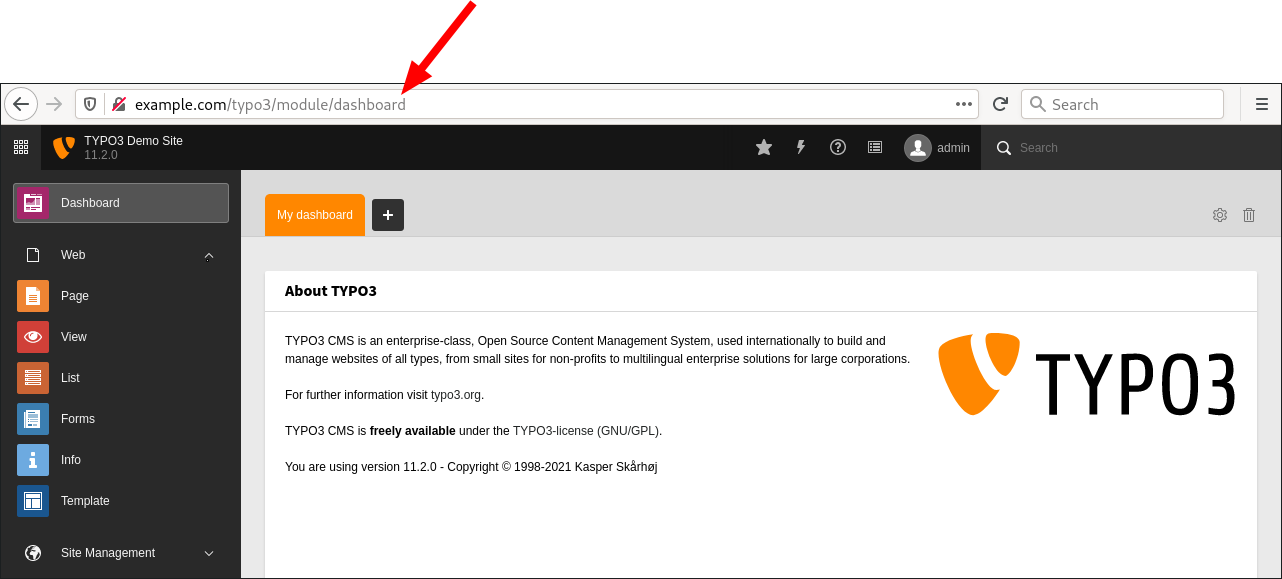
\includegraphics[width=0.85\linewidth]{BackendUserInterface/1618653909-DeepLinkingInTheBackend.png}
	\end{figure}

\end{frame}

% ------------------------------------------------------------------------------

\begin{frame}[fragile]
	\frametitle{Interface Utilisateur Backend}
	\framesubtitle{Liens directs dans le Backend (2)}

	Quelques exemples de liens directs~:
	\vspace{0.2cm}
	\begin{itemize}
		\item (Pré)visualisation de page (ID=123)~:\newline
			\fontsize{8}{10}\texttt{https://example.com/typo3/module/web/ViewpageView?id=123}\normalsize
		\item Édition de la configuration de site~:
			\fontsize{8}{10}\texttt{https://example.com/typo3/module/site/configuration?action=edit}\normalsize
		\item Édition d'un élément de contenu (ID=42)~:
			\fontsize{8}{10}\texttt{https://example.com/typo3/record/edit?edit[tt\_content][42]=edit}\normalsize
		\item Ouverture du module «~Utilisateurs Backend~»~:
			\fontsize{8}{10}\texttt{https://example.com/typo3/module/system/BeuserTxBeuser}\normalsize
	\end{itemize}

\end{frame}

% ------------------------------------------------------------------------------
